\documentclass[12pt,titlepage]{article}

\usepackage{geometry}
\geometry{
    a4paper,
    total={210mm,297mm},
    left=20mm,
    right=20mm,
    top=20mm,
    bottom=20mm,
}

	
\usepackage[]{subcaption}

\usepackage{pdflscape}

\usepackage{graphicx}
\usepackage{subcaption}

% Polski
\usepackage[]{polski} 
\usepackage[polish]{babel}

%do tabel
\usepackage{multirow}

% Pierwszy akapit - wcięty
\usepackage[]{indentfirst}

% Matematyka
\usepackage[]{amsfonts}

\usepackage[]{amsmath}

% Formatowanie
\usepackage{ragged2e}

% Tytuły sekcji
\usepackage{titlesec}
%\titleformat{\section}[block]{\Large\bfseries}{}{1em}{}

% <=
\usepackage{amssymb}

% eps
\usepackage{graphicx}
% \usepackage{subfigure}

% Tabele
\usepackage{array}

\usepackage[style=czech]{csquotes}

\renewcommand*{\thesubsubsection}{}

\usepackage{hyperref}
\hypersetup{
    colorlinks,
    citecolor=black,
    filecolor=black,
    linkcolor=black,
    urlcolor=black
}

\usepackage[numbered]{matlab-prettifier}
\lstset{
    literate={ą}{{\k{a}}}1
    {Ą}{{\k{A}}}1
    {ę}{{\k{e}}}1
    {Ę}{{\k{E}}}1
    {ó}{{\'o}}1
    {Ó}{{\'O}}1
    {ś}{{\'s}}1
    {Ś}{{\'S}}1
    {ł}{{\l{}}}1
    {Ł}{{\L{}}}1
    {ż}{{\.z}}1
    {Ż}{{\.Z}}1
    {ź}{{\'z}}1
    {Ź}{{\'Z}}1
    {ć}{{\'c}}1
    {Ć}{{\'C}}1
    {ń}{{\'n}}1
    {Ń}{{\'N}}1
}

\title{

\includegraphics[scale=0.75]{img/politechnika_sl_logo_bw_poziom_pl.eps}\\
\textbf{Wydział Automatyki, Elektroniki\\
i Informatyki}\\
\vspace*{1cm}
Systemy Interaktywne i Multimedialne \\ Projekt \\ Detekcja emocji w głosie

\vspace*{5cm}
}
\author{
Natalia Stręk
Jakub Kula,
Paweł Wójtowicz,
} 
\date{Gliwice 2023}

\begin{document}

\maketitle

\tableofcontents

\newpage
\section{Cele i zadania z okresu maj}
% Cele i zadania z okresu objętego sprawozdaniem, których realizację już podjęto. Należy odnieść się do zaakceptowanego dokumentu Informacje o realizowanym projekcie (ok 100 słów)\\
Głónym celem na maj było stworzono UI pozwalające na wybranie pliku dźwiękowego oraz nagranie wiadomości głosowej, używając Tkinter, z którego zostają wyciąganięte parametry służące do predykcji emocji. Celem dodatkowym była ciągła praca nad siecią neruonową w celu poprawy doładności na zbiorze tesotwym.

\section{Opis zadań przyjętych do realizacji}
Do tego momentu zostały zrealizowane następujące zadania
\begin{itemize}
    \item Zgromadzenie i przetworzenie danych - dane w postaci krótkich nagrań dźwiękowych reprezentujące różne emocje,
    \item Wybór oraz ekstrakcja cech,
    \item Wybór architektury sieci, hiperparametrów, podział danych na zbiór uczący oraz treningowy,
    \item Trenowanie modelu i optymalizacja parametrów modelu,
    \item Ocena i walidacja modelu.
\end{itemize}

A następujące zadania zostały przyjęte do realizacji:
\subsubsection{Stowrzenie UI}
UI jest zaprojektowane w sposób intuicyjny, umożliwiając użytkownikom łatwe dodanie pliku dźwiękowego oraz nagranie własnej wiadomości przy użyciu wbudowanego mikrofonu.

\begin{figure}[ht]
    \centering
    \begin{subfigure}[b]{0.3\textwidth}
        \centering
        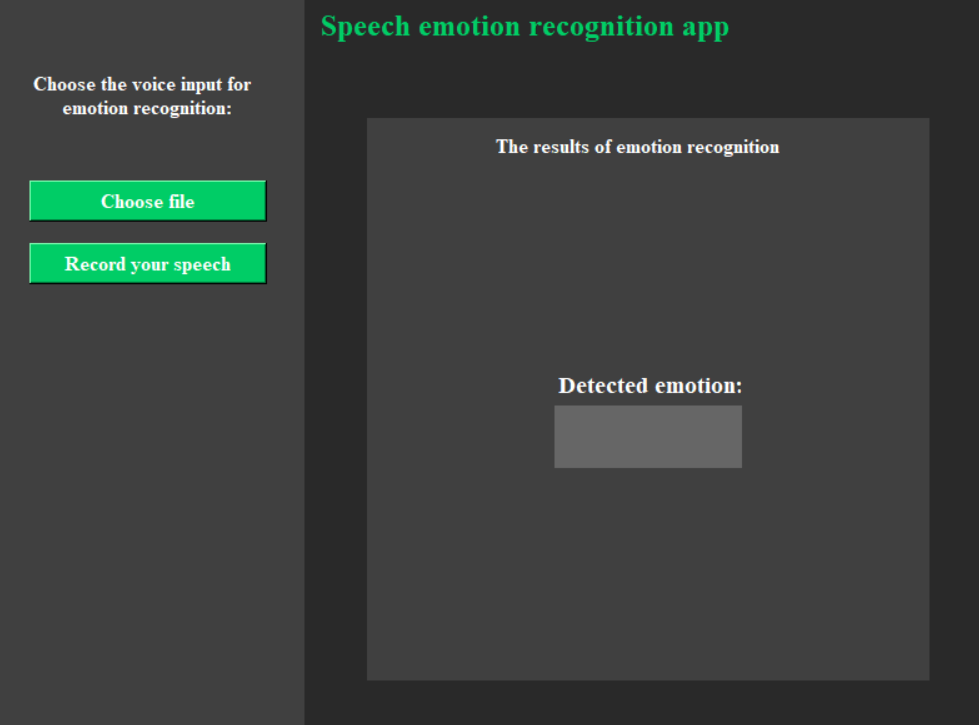
\includegraphics[width=\textwidth]{img/1.png}
        \label{fig:sub1}
    \end{subfigure}
    \hfill
    \begin{subfigure}[b]{0.3\textwidth}
        \centering
        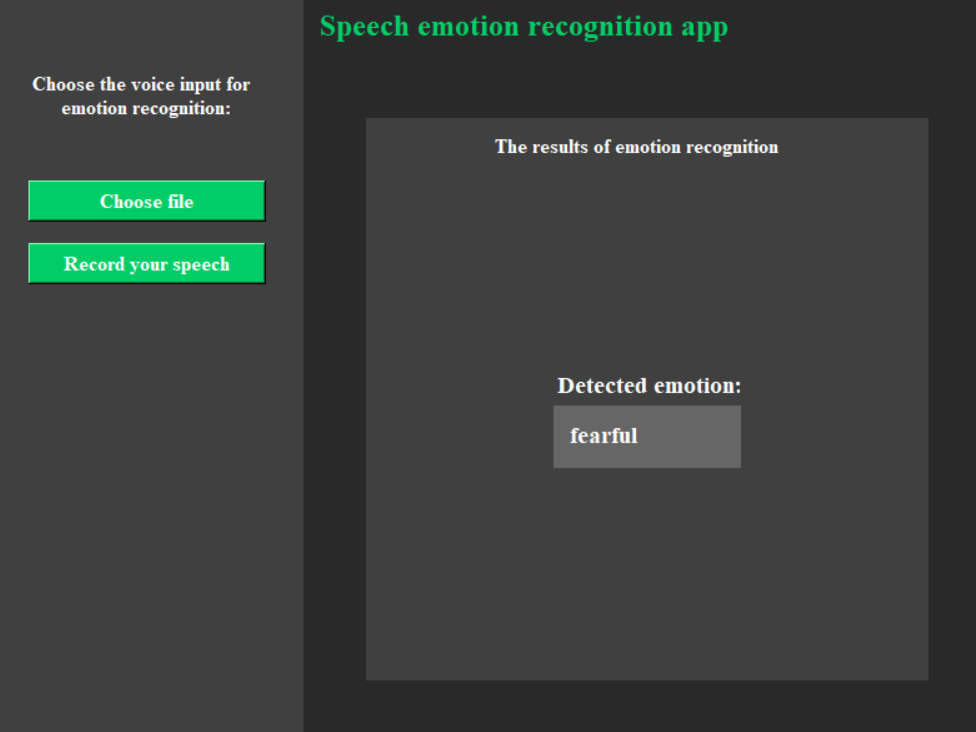
\includegraphics[width=\textwidth]{img/2.png}
        \label{fig:sub2}
    \end{subfigure}
    \hfill
    \begin{subfigure}[b]{0.3\textwidth}
        \centering
        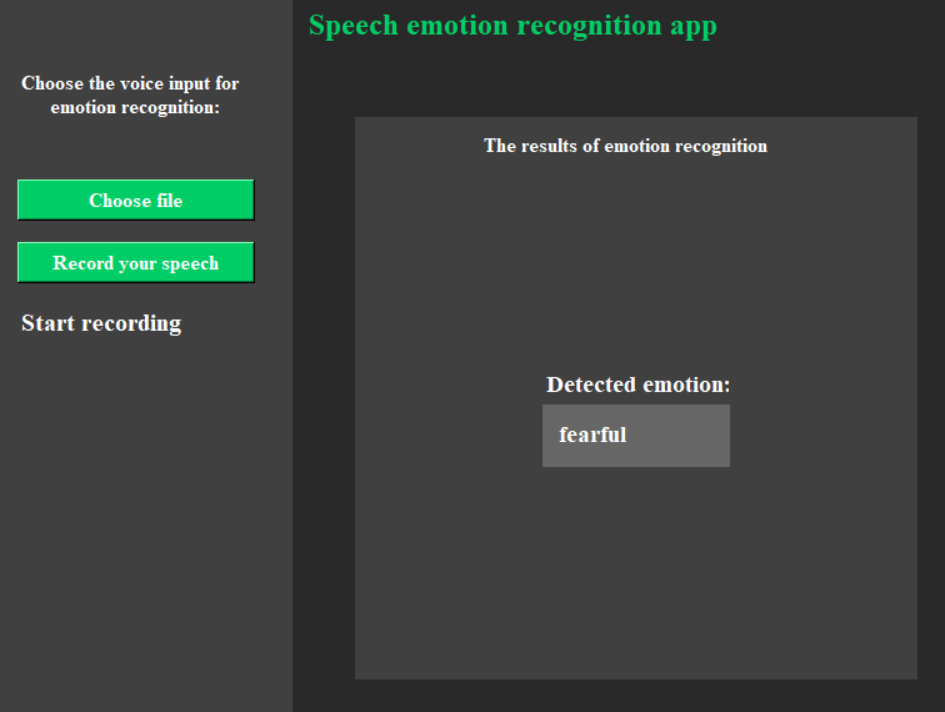
\includegraphics[width=\textwidth]{img/3.png}
        \label{fig:sub3}
    \end{subfigure}
    \label{fig:main}
\end{figure}
Prace nad interfejsem użytkownika są w toku. Dotychczas stworzono pierwszy zarys UI, który umożliwia użytkownikom dodawanie plików dźwiękowych oraz nagrywanie wiadomości za pomocą wbudowanego mikrofonu. Interfejs jest zaprojektowany tak, aby był intuicyjny i łatwy w obsłudze. Na obecnym etapie prace nad UI są zaawansowane w 80\%. Planowane są dalsze udoskonalenia, w tym integracja z modelem analizy emocji oraz poprawa responsywności i estetyki interfejsu. Celem jest zapewnienie użytkownikom wygodnego i efektywnego narzędzia do interakcji z systemem.


\subsubsection{Poprawa dokładność sieci}
W ramach prac nad dokładnością modelu, zostały wykonane testy optymaliacji hiperparametrów sieci.Proces dostosowywania parametrów modelu jest kluczowym krokiem w optymalizacji jego wydajności. Obejmuje to fine-tuning hiperparametrów, takich jak współczynnik uczenia, liczba neuronów w warstwach ukrytych oraz liczba epok treningowych. Dotychczasowe testy sugerują, że dostosowanie tych parametrów może znacząco poprawić dokładność modelu w rozpoznawaniu emocji. Wykazały one, że zwiększeni skomplikowania modelu, spowodowało zmniejszenie biasu, co poskutkowało znacznie lepszymi wynikami kroswalidacji. Obecny najlepszy model osiąga wartośc 76\% dokładności na zbiorze testowym.
\begin{center}
    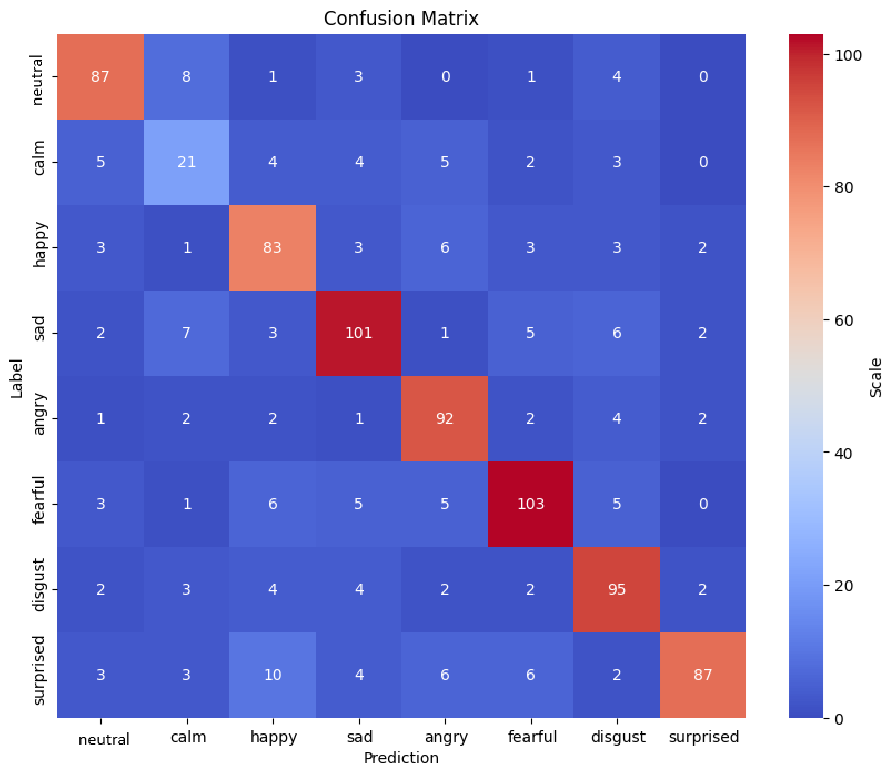
\includegraphics[width=\textwidth]{img/conf_matrix.png}
\end{center}
Można zauważyć, że nowy model znacząco lepiej radzi sobie z klasyfikacją emocji w głosie. Różnica w ilości cech w zbiorze testowym dla emocji "calm" wynika z wybranych zbiorów nagrań głosowych. Pierwszy z nich posiadał 8, a drugi, większy, tylko 7.\\ Dostosowywanie parametrów w celu poprawy wydajności modelu jest zadaniem najbardziej czasochłonnym, które wymagało około tygodnia pracy.

\section{Zgodność z harmonogramem}
Projekt jest realizowany zgodnie z harmonogramem
\section{Czy wprowadzono znaczące zmiany do projektu?}
Nie wprowadzono w tym etapie żadnych znaczących zmian odbiegających od harmongoramu projektu.


\end{document}